%%%%%%%%%%%%%%%%%%%%%%%%%%%
% Práctica 4:  Diseño arquitectónico de una Aplicación 
% @uthor: Alejandro David Arzola Saavedra
% @date: 15/10/2023
%%%%%%%%%%%%%%%%%%%%%%%%%%%
% Estructura basica de la pagina
\documentclass[a4paper]{article}
\usepackage[utf8]{inputenc}
\usepackage[spanish]{babel}
\usepackage{fancyhdr} %Definimos el estilo de página

% Paquetes adicionales
\usepackage{graphicx,efbox}
\usepackage[headsep=0.2cm]{geometry}
\usepackage[most]{tcolorbox}
\newcommand{\MYhref}[3][black]{\href{#2}{\color{#1}{#3}}}
\usepackage[hyperindex=true, colorlinks=true, linkcolor=black, breaklinks=true, urlcolor=black, citecolor=black, anchorcolor= black]{hyperref}


% Agrega el paquete para personalizar el índice
\usepackage{tocloft}

% Personaliza la apariencia de la entrada "Bibliografía" en el índice
\renewcommand{\cftsecleader}{\cftdotfill{\cftdotsep}}
\renewcommand{\cftsecafterpnum}{\vspace{0.5\baselineskip}}



% Variable de entorno de fecha
\newcommand{\dateToday}{15 de octubre de 2023}

% Variable de imagenes
\newcommand{\logoULPGC}{imagenes/ulpgc.png}
\newcommand{\portada}{imagenes/arquitectura.PNG}
\newcommand{\mvvm}{imagenes/mvvm.png}
\newcommand{\mvp}{imagenes/mvp.png}
\newcommand{\hexagonal}{imagenes/hexagonal.png}
\newcommand{\cleanArchitecture}{imagenes/cleanArchitecture.png}
\newcommand{\mvpModel}{imagenes/mvp_model.png}
\newcommand{\cleanArch}{imagenes/CleanArchitecture.jpg}

%Cambio indice
\addto\captionsspanish{\renewcommand{\contentsname}{Índice}}

\setlength{\headheight}{ 40.2pt}
\pagestyle{fancy}
\lhead{\includegraphics[width=5cm]{\logoULPGC}}
\rhead{
\includegraphics[height=1cm]{imagenes/programador.png}}

\geometry{a4paper, total={170mm,257mm}, left=35mm, top=20mm, right=35mm}

\begin{document}
    %%%%%%%%%%%%%%%%%%%%%%%%%%%%%%%%%
    %%   Portada del documento
    %%%%%%%%%%%%%%%%%%%%%%%%%%%%%%%%%
    \begin{titlepage}
        \centering
        \vspace*{2cm}

        \includegraphics[width=0.6\textwidth]{\logoULPGC}\par\vspace{1cm}
    
        {\scshape\textbf{\LARGE Práctica 4}}\par
        \vspace{0.6cm}
        {\bfseries}{\Huge Elección de una arquitectura}
        \vspace{1cm}


            \centering
            \fbox{\includegraphics[width=\textwidth, height=8cm, keepaspectratio]{\portada}}
            \vspace{1cm}

        
        \begin{tcolorbox}[colback=red!5!white,colframe=white!50!black]
            \centering \Large Programación de Aplicaciones Móviles Nativas \par
            \dateToday
        \end{tcolorbox}

        \vspace{1cm}        
        \begin{tcolorbox}[colback=blue!5!white,colframe=blue!75!black]
            Autor:
            \tcblower
            Alejandro David Arzola Saavedra (alejandro.arzola101@alu.ulpgc.es)
        \end{tcolorbox}
    \end{titlepage}
    
    \newpage
        
    %%%%%%%%%%%%%%%%%%%%%%%%%%%%%%%%%
    % Tabla de contenido de la pagina
    %%%%%%%%%%%%%%%%%%%%%%%%%%%%%%%%%
    \tableofcontents 
    
    \newpage

    %%%%%%%%%%%%%%%%%%%%%%%%%%%
    % Introduccion de la pagina
    %%%%%%%%%%%%%%%%%%%%%%%%%%%
    \section{Introducción}

    Se presentan cinco supuestos prácticos relacionados con el desarrollo de aplicaciones móviles. Cada supuesto tiene sus propias restricciones y requisitos, como presupuesto, tiempos de entrega y hay que  justificar qué arquitectura es la más adecuada para cada supuesto
    
    %%%%%%%%%%%%%%%%%%%%%%%%%%%
    % Desarrollo de la pagina
    %%%%%%%%%%%%%%%%%%%%%%%%%%%
    \section{Desarrollo} 
    
    %%%%%%%%%%%%%%%%%%%%%%%%%%%
    % Supuesto 1
    %%%%%%%%%%%%%%%%%%%%%%%%%%%
    \subsection{Supuesto 1: Aplicación de E-commerce para una PYME}
    
    Una pequeña empresa quiere lanzar su tienda online a través de una \textbf{aplicación móvil nativa}.\vspace{0.2cm}
    
    \textbf{Presupuesto}: Limitado.\vspace{0.2cm}
    
    \textbf{Tiempos de entrega}: 4 meses.\vspace{0.2cm}
    
    \textbf{Recursos humanos}: Un desarrollador principal y un diseñador.\vspace{0.2cm}
    
    \textbf{Rendimiento}: Tráfico moderado, es esencial que la aplicación sea rápida y eficiente.\vspace{0.2cm}

    \subsubsection{Selección de la Arquitectura}
    
    Para una aplicación comentada previamente aunque \textbf{MVC es comúnmente utilizado y menos complejo}, para el contexto de \textbf{aplicaciones móviles nativas}, la arquitectura \textbf{MVVM} (Model-View-ViewModel) podría ser \textbf{la opción más apropiada} para 4 meses de desarrollo.\vspace{0.3cm}

    \textbf{MVC}, en su concepción, se aplicó principalmente a aplicaciones de escritorio y web, \textbf{no considerando específicamente las peculiaridades de las aplicaciones móviles nativas}.\vspace{0.3cm}
    
    La elección de \textbf{MVVM conlleva varias ventajas}. En primer lugar, ofrece una clara \textbf{separación de responsabilidades}, lo cual es fundamental para un \textbf{desarrollo eficiente}, especialmente cuando se cuenta con \textbf{un solo desarrollador y un presupuesto limitado}. La capacidad de \textbf{enlace de datos bidireccional} de MVVM facilita la \textbf{actualización dinámica de la interfaz de usuario}, proporcionando una \textbf{experiencia fluida y agradable para el usuario}.\vspace{0.3cm}
    
    La \textbf{facilidad de mantenimiento} es otra ventaja significativa. Al \textbf{separar las responsabilidades} entre el modelo, la vista y el modelo de vista, se \textbf{simplifica la gestión del código}, lo cual es crucial en \textbf{equipos pequeños}.\vspace{0.3cm}
    
    Además, \textbf{MVVM} contribuye a mejorar la \textbf{experiencia del usuari}o al permitir una \textbf{interfaz más receptiva y dinámica}. En un entorno de E-commerce, donde \textbf{la velocidad y la fluidez son esenciales}, esta capacidad puede marcar la diferencia.\vspace{0.3cm}
    
    \textbf{Comparando con otras arquitecturas}, como la \textbf{hexagonal} o \textbf{clean architecture}, que pueden ser \textbf{más complejas y quizás excesivas para un único desarrollador con un tráfico moderado}, \textbf{MVVM se presenta como una opción más adecuada} para el caso específico.

    \begin{center}
        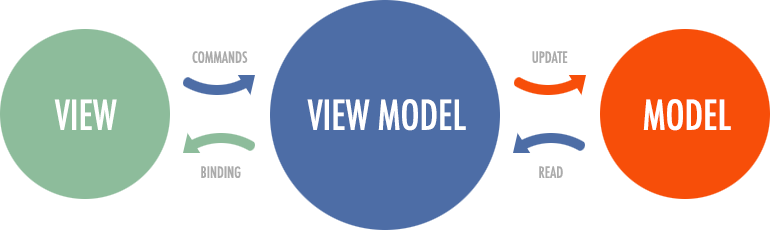
\includegraphics[width=\textwidth, height=5cm, keepaspectratio]{\mvvm}\vspace{0.2cm}\par
        \textbf{Imagen 1: Arquitectura MVVM}
    \end{center}

    %%%%%%%%%%%%%%%%%%%%%%%%%%%
    % Supuesto 2
    %%%%%%%%%%%%%%%%%%%%%%%%%%%        
    \subsection{Supuesto 2: Aplicación Social Interactiva para una Startup}

    Una startup quiere crear una aplicación social con características interactivas, como chats en tiempo real y transmisiones en vivo.\vspace{0.2cm}

    \textbf{Presupuesto}: Moderado.\vspace{0.3cm}

    \textbf{Tiempos de entrega}: 6-8 meses.\vspace{0.2cm}
    
    \textbf{Recursos humanos}: Tres desarrolladores, un diseñador y un programador backend.\vspace{0.2cm}
    
    \textbf{Rendimiento}: Alto tráfico y crucial que maneje interacciones en tiempo real.\vspace{0.2cm}
    
    \subsubsection{Selección de la Arquitectura}

    En el contexto de una aplicación social con \textbf{chats en tiempo real}, donde contamos con un presupuesto moderado y un plazo de desarrollo de 6 a 8 meses, la elección de utilizar \textbf{MVP con Clean Architecture} emerge como una opción sólida y bien fundamentada.\vspace{0.3cm}

    Dada la naturaleza interactiva de la aplicación, especialmente con funciones de \textbf{chat en tiempo real y transmisiones en vivo}, \textbf{el modelo MVP proporciona una clara separación de responsabilidades} entre el Modelo, la Vista y el Presentador. Esta división es esencial para \textbf{gestionar flujos de datos reactivos y permitir cambios frecuentes en la lógica de presentación}.\vspace{0.3cm}
    
    El Presentador en el modelo MVP juega un papel central al manejar las interacciones y actualizar la interfaz de usuario en tiempo real. Esto es crucial para \textbf{ofrecer una experiencia fluida a los usuarios, especialmente en un entorno social donde la interactividad es clave}.\vspace{0.3cm}
    
    La incorporación de \textbf{Clean Architetecture} \textbf{refuerza la independencia entre capas}, lo cual es esencial para \textbf{adaptarse a cambios rápidos en los requisitos}, una realidad común en startups. La flexibilidad que proporciona Clean Architecture facilita \textbf{la adición de nuevas características y modificaciones sin impactar negativamente en otras partes del sistema}.\vspace{0.3cm}
    
    Considerando el tiempo y presupuesto moderados, la elección de \textbf{MVP} se alinea con \textbf{un enfoque más liviano en comparación con arquitecturas más complejas}. La combinación de MVP con Clean Architecture establece una base \textbf{robusta para la escalabilidad}, preparando la aplicación para crecimientos futuros.\vspace{0.3cm}
    
    La optimización para el \textbf{alto tráfico}, especialmente en el caso de chats en tiempo real, es \textbf{facilitada por la estructura de MVP} cuando se combina con tecnologías adecuadas. Este enfoque no solo es \textbf{eficiente en términos de rendimiento}, sino que también respalda una \textbf{experiencia de usuario efectiva}, un factor clave para \textbf{mantener la satisfacción de los usuarios} en una aplicación social interactiva.\vspace{0.3cm}
    


    \begin{center}
        \includegraphics[width=0.45\textwidth, height=10cm, keepaspectratio]{\mvpModel}
        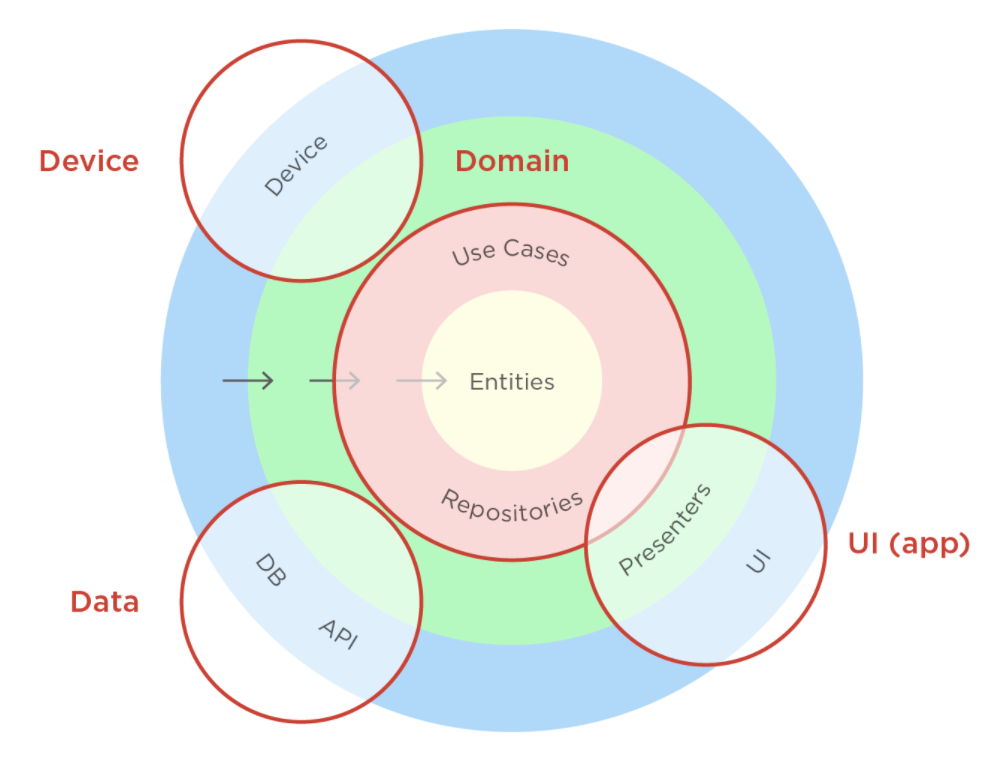
\includegraphics[width=0.4\textwidth, height=10cm, keepaspectratio]{\cleanArchitecture}
        \vspace{0.2cm}\par\textbf{Imagen 2: Arquitectura MVP y Clean Architecture}\label{fig:imagen-captura-estilo-pagina}
    \end{center}
    \newpage
    
    \subsection{Supuesto 3: Aplicación Financiera para una Gran Empresa}

    Una gran empresa financiera quiere desarrollar una aplicación para que sus clientes gestionen sus finanzas, con características como visualización de transacciones, transferencias y análisis financiero.\vspace{0.2cm}
    
    \textbf{Presupuesto}: Alto.\vspace{0.2cm}
    
    \textbf{Tiempos de entrega}: 10-12 meses.\vspace{0.2cm}
    
    \textbf{Recursos humanos}: Un equipo grande con múltiple desarrolladores, diseñadores, especialistas en seguridad y analistas.\vspace{0.2cm}
    
    \textbf{Rendimiento}: Tráfico muy alto y es esencial que la aplicación sea segura y eficiente.\vspace{0.2cm}

    \subsubsection{Selección de la Arquitectura}
    
    Con un amplio presupuesto, un extenso plazo de entrega y la presencia de un equipo numeroso de desarrolladores y especialistas en seguridad, la elección más apropiada sería la implementación de \textbf{Clean Architecture}.\vspace{0.3cm}
    
    La prioridad aquí es \textbf{la seguridad de los datos}, y \textbf{Clean Architecture} proporciona una estructura que permite una \textbf{clara separación entre las capas}, facilitando así \textbf{la implementación de medidas de seguridad sólidas}. En este contexto, \textbf{la capa de negocio puede ser diseñada específicamente para contener tanto la lógica empresarial como las reglas de seguridad}.\vspace{0.3cm}
    
    Aunque Clean Architecture implica una \textbf{inversión inicial} de tiempo debido a su \textbf{enfoque modular}, es particularmente \textbf{adecuada para proyectos a largo plazo con un presupuesto significativo}. Su facilidad de \textbf{mantenimiento y escalabilidad} a medida que evolucionan los requisitos la convierten en una elección acertada.\vspace{0.3cm}
    
   Con Clean Architecture se \textbf{simplifica la colaboración entre especialistas}, ya que cada grupo puede \textbf{enfocarse en su área sin interferencias innecesarias}.\vspace{0.3cm}
    
    En rendimiento, la estructura modular contribuye a \textbf{optimizar el rendimiento} de la aplicación, \textbf{mejorando su capacidad para gestionar altos volúmenes de tráfico}.\vspace{0.3cm}
    
    La fortaleza de Clean Architecture se utiliza cuando se espera un crecimiento sustancial de la aplicación. Permite la \textbf{adición de nuevas características sin afectar el sistema existente}, lo que es \textbf{crucial en proyectos a gran escala con un presupuesto generoso}.\vspace{0.3cm}
    
    En comparación con MVP o MVI, \textbf{Clean Architecture} destaca como una \textbf{elección preferida en escenarios donde los recursos no son una limitación}.\vspace{0.3cm} 
    
    Si se implementa adecuadamente, Clean Architecture puede ofrecer una \textbf{experiencia de usuario eficiente y segura}. 

    \begin{center}
        \includegraphics[width=\textwidth, height=6.5cm, keepaspectratio]{\cleanArch}\vspace{0.2cm}\par
        \textbf{Imagen 3: Clean architecture}
    \end{center}

    
    \newpage

    %%%%%%%%%%%%%%%%%%%%%%%%%%%
    % Supuesto 4
    %%%%%%%%%%%%%%%%%%%%%%%%%%%
    \subsection{Supuesto 4: Plataforma de Salud y Bienestar para Hospitales}

    Un hospital de renombre desea desarrollar una aplicación móvil nativa que permita a los pacientes acceder a sus historiales médicos, programar citas, chatear con especialistas y recibir recomendaciones personalizadas basadas en su historial.\vspace{0.2cm}
    
    \textbf{Presupuesto}: muy alto.\vspace{0.2cm}
    
    \textbf{Tiempos de entrega}: 12-15 meses.\vspace{0.2cm}
    
    \textbf{Recursos humanos}: un equipo multidisciplinario compuesto por varios desarrolladores móviles, desarrolladores backend, especialistas en seguridad de la información, diseñadores UX/UI y analistas de sistemas.\vspace{0.2cm}
    
    \textbf{Rendimiento}: se espera un tráfico constante y alto debido a la gran cantidad de pacientes. La seguridad y privacidad de los datos es primordial.
    
    \subsubsection{Selección de la Arquitectura}
    
    En este escenario, donde contamos con un \textbf{equipo multidisciplinario} y un \textbf{plazo extenso para el desarrollo de la aplicación}, con un enfoque prioritario en la seguridad, la elección de la A\textbf{rquitectura Hexagonal se presenta como una opción sólida}.\vspace{0.3cm}

    La \textbf{Arquitectura Hexagonal} se destaca por su enfoque en la \textbf{separación de capas}, lo que resulta beneficioso para la \textbf{implementación de medidas de seguridad}. Al establecer límites claros entre capas, la Arquitectura Hexagonal \textbf{controla el acceso a los datos, fortaleciendo la seguridad de la aplicación}.\vspace{0.3cm}
    
    Dado que disponemos de un presupuesto alto y un plazo de entrega considerable, la Arquitectura Hexagonal se \textbf{adapta bien a este contexto}, aunque requiere más tiempo y recursos, \textbf{especialmente en las etapas iniciales}, \textbf{para establecer la separación de responsabilidades de manera efectiva} al final acaba siendo la mas conveniente en \textbf{aplicaciones a largo plazo}.\vspace{0.3cm}
    
    La mantenibilidad a largo plazo se ve favorecida por esta arquitectura, aprovechando \textbf{la colaboración entre especialistas de diversas áreas en un equipo multidisciplinario}. La Arquitectura Hexagonal \textbf{facilita la interacción entre desarrolladores} móviles, backend y expertos en seguridad, entre otros.\vspace{0.3cm}
    
    En términos de \textbf{rendimiento}, la Arquitectura Hexagonal muestra eficiencia al \textbf{separar la lógica de negocio y las capas}, lo que contribuye a un mejor rendimiento.\vspace{0.3cm}
    
    La Arquitectura Hexagonal se distingue por su \textbf{facilidad para escalar}. A medida que la plataforma crece, \textbf{se pueden agregar nuevas funcionalidades e introducir nuevos adaptadores sin afectar la lógica de negocio}, lo que simplifica el proceso de expansión.\vspace{0.3cm}
    
    La \textbf{modularidad} y la clara \textbf{separación de responsabilidades} ofrecidas por la Arquitectura Hexagonal \textbf{facilitan el desarrollo de interfaces eficientes y libres de errores}.
    
    \begin{center}
        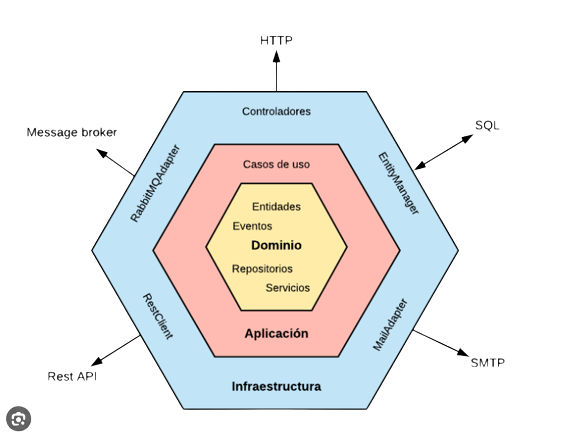
\includegraphics[width=\textwidth, height=6.5cm, keepaspectratio]{\hexagonal}\vspace{0.2cm}\par
        \textbf{Imagen 4: Arquitectura hexagonal}
    \end{center}

    \newpage

    %%%%%%%%%%%%%%%%%%%%%%%%%%%
    % Supuesto 5
    %%%%%%%%%%%%%%%%%%%%%%%%%%%
    \subsection{Supuesto 5: Aplicación Prototipo para un Hackathon}

    Un grupo de estudiantes decide participar en un hackathon de 48 horas. Su objetivo es crear un prototipo funcional de una aplicación móvil que ayude a las personas a encontrar compañeros de viaje para compartir gastos en carreteras de
    peaje.\vspace{0.2cm}
    
    \textbf{Presupuesto}: Mínimo. Los estudiantes usarán herramientas y recursos gratuitos.\vspace{0.2cm}
    
    \textbf{Tiempos de entrega}: 48-72 horas.\vspace{0.2cm}
    
    \textbf{Recursos humanos}: Tres estudiantes con habilidades mixtas: un desarrollador, un diseñador y alguien con habilidades de negocio.\vspace{0.2cm}
    
    \textbf{Rendimiento}: Como es un prototipo, no se espera un tráfico real. La aplicación debe ser lo suficientemente funcional para demostrar la idea.\vspace{0.2cm}

    \subsubsection{Selección de la Arquitectura}
    
    Nos encontramos con un grupo de estudiantes inmersos en un hackatón donde los \textbf{recursos son limitados, el tiempo es escaso y solo contamos con un desarrollador}. En este contexto, la elección más adecuada podría ser la implementación del patrón de \textbf{arquitectura MVP} (Model-View-Presenter).\vspace{0.3cm}

    MVP es una de las arquitecturas más comunes y, en este caso, su \textbf{simplicidad}, \textbf{rapidez de implementación} pueden ser ventajas significativas. Dada la \textbf{falta de experiencia laboral del equipo}, la estructura clara de \textbf{MVP} permite que \textbf{cada miembro del equipo se enfoque en su área de especialización}.\vspace{0.3cm}
    
    Al asignar al desarrollador \textbf{la lógica de negocio}, al diseñador \textbf{la responsabilidad de trabajar en la vista}, y a la persona con \textbf{habilidades en el negocio} colaborar en la lógica de presentación,\textbf{las fortalezas individuales del equipo se potenciarán}. Además, \textbf{MVP} \textbf{facilita la interactividad y la gestión de eventos de usuario}, aspectos fundamentales para demostrar la aplicación en el hackatón.\vspace{0.3cm}
    
    La simplicidad de \textbf{MVP} también permite \textbf{adaptarse fácilmente a cambios rápidos}, una característica crucial en un entorno de hackatón donde los \textbf{requisitos pueden evolucionar rápidamente}. Al no permitir que la vista interactúe directamente con el modelo, \textbf{las modificaciones en la interfaz no afectarán sustancialmente la lógica de negocio}, permitiendo iteraciones más rápidas.\vspace{0.3cm}
    
    En un hackatón, donde el tiempo de entrega es muy limitado (entre 2 y 3 días) y \textbf{no se busca un diseño altamente perfeccionado}, \textbf{MVP} destaca por su \textbf{capacidad para mejorar la experiencia del usuario}.\vspace{0.3cm}
    
    En cuanto a la escalabilidad, es cierto que \textbf{MVP} puede \textbf{tener limitaciones en comparación con algunas arquitecturas más complejas}. Sin embargo, para el contexto del hackatón, ofrece una \textbf{solución suficientemente escalable}. \textbf{Si la aplicación evoluciona en el futuro, se pueden explorar opciones más escalables y robustas}.\vspace{0.3cm}
    
    \begin{center}
        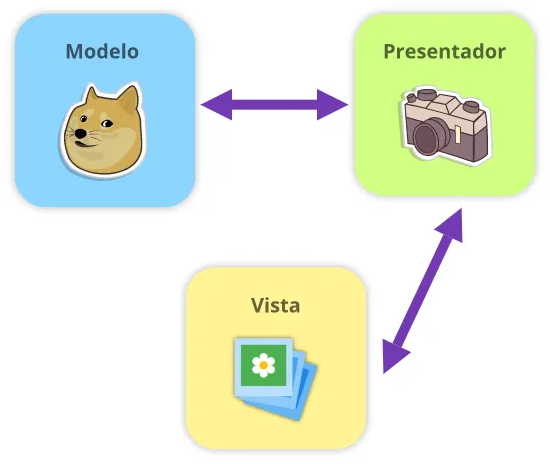
\includegraphics[width=\textwidth, height=5cm, keepaspectratio]{\mvp}\vspace{0.2cm}\par
        \textbf{Imagen 5: Arquitectura MVP}
    \end{center}

    \section{Conclusión}
    Como hemos observado, la elección de la arquitectura adecuada para un proyecto depende de varios factores, incluyendo las \textbf{necesidades específicas y los recursos disponibles}.\vspace{0.3cm}

    La ventaja de esta diversidad de patrones de arquitectura es que brinda \textbf{opciones variadas para abordar distintos tipos de aplicaciones}. La \textbf{habilidad para seleccionar la arquitectura más adecuada} es fundamental para el \textbf{éxito de un proyecto}.\vspace{0.3cm}
    
    En última instancia, la clave reside en \textbf{tomar decisiones informadas} sobre la arquitectura, basadas en las particularidades y requisitos específicos de cada proyecto.\vspace{0.3cm}
        
    %%%%%%%%%%%%%%%%%%%%%%%%%%%
    % Bibliografia de la pagina
    %%%%%%%%%%%%%%%%%%%%%%%%%%%
    \addcontentsline{toc}{section}{4\hspace{0.4cm}Bibliografía}
    \renewcommand{\refname}{4.\hspace{0.6cm}Bibliografía}
    
    \begin{thebibliography}{9}
        \bibitem{mvc} MVC en android. Recuperado de \url{https://fahedhermoza.medium.com/por-qu%C3%A9-no-funciona-mvc-en-android-d0b747a823c0}
        
        \bibitem{hexagonal} Arquitectura hexagonal. Recuperado de \url{https://blog.hubspot.es/website/que-es-arquitectura-hexagonal}
    
        \bibitem{clean} Clean Architecture .Recuperado de \url{https://wahibhaq.com/blog/clean-architecture-mvp-summary/}
        
        \bibitem{mvp} MVP en android. Recuperado de \url{https://medium.com/@carloslopez_19744/%EF%B8%8F-arquitectura-mvp-en-android-para-principiantes-30b5675ff7b6}

        \bibitem{hex} Arquitectura hexagonal. Recuperado de \url{https://medium.com/@edusalguero/arquitectura-hexagonal-59834bb44b7f}

        \bibitem{clear} Clean Software. Recuperado de \url{https://www.linkedin.com/pulse/clean-software-architecture-key-performance-security-mariam-waheed/}
        
        
    \end{thebibliography}
\end{document}